\chapter{\LaTeX{} : définition et intérêts}

\begin{prealable}
 Dans ce chapitre nous allons vous présenter brièvement \LaTeX{} et les raisons pour lesquelles nous pensons que son apprentissage est utile pour la rédaction de travaux en sciences humaines.
\end{prealable}

\section{Pourquoi \LaTeX{} ?}

\subsection{Inconvénient des traitements de textes}

Quand vous rédigez un texte dans votre traitement de texte, comme par exemple Microsoft Word ou Openoffice.org, celui-ci exécute deux actions simultanées :

\begin{itemize}
\item D'une part il stocke dans un fichier la structure logique de votre texte : titres, paragraphes, notes de bas de pages etc.
\item D'autre part il vous affiche à l'écran le rendu \enquote{physique} de votre texte (justifications, gras, italiques etc), tel qu'un lecteur en disposera.
\end{itemize}

Pour cette raison on appelle ce type de logiciel WYSIWYG, ce qui en anglais signifie \textenglish{What You See Is What You Get}\footnote{\enquote{Ce que vous voyez est ce que vous faites}.}. 

Cette combinaison de deux fonctions différentes dans les  traitements de texte a trois conséquences :

\begin{itemize}
\item La nécessité d'afficher en temps réel le rendu physique du texte tout en conservant une vitesse relativement élevée du logiciel entraîne une baisse de la qualité typographique. Par exemple :
	\begin{itemize}
		\item Pour avoir un texte justifié à gauche et à droite, les traitements de texte font varier la taille des espaces entre les mots. Les variations peuvent parfois être considérables ce qui peut diminuer le confort de lecture. Pour éviter ce type d'ennui, les livres \enquote{classiques} coupent les mots en fin de ligne, ce qu'on appelle une césure\footnote{La césure ne se fait toutefois pas n'importe où : elle doit respecter des règles propres à chaque langue.}.
		\item Les blancs situés avant certains signes de ponctuations, comme par exemple les points d'exclamation font la même taille que les blancs séparant les mots, alors que les règles typographiques \enquote{classiques} prévoient des blancs plus petits.
	\end{itemize}
\item Le fait qu'un même logiciel s'occupe \emph{à la fois} de l'affichage et de la structure du texte incite à confondre les deux. Ce qui peut avoir deux effets négatifs, qui ne sont pas systématiques toutefois\footcite[Les auteurs de ces lignes sont moins sévères envers les traitements de texte que d'autres LaTeXiens : \cf][]{stupide}:
	\begin{itemize}
		\item Cela peut inciter à se concentrer sur le forme plutôt que sur le fond et la structure. Toutefois en théorie la formation universitaire de sciences humaines incite à penser \emph{structure et sens d'abord}\footcite[Voir un débat sur le blog d'un des auteurs]{structurevsforme}. 
		\item Les rédacteurs n'utilisent pas toujours la possibilité de séparer sens et forme grâce aux styles. Dans ces cas, lorsqu'on désire changer la forme d'un élément logique (par exemple le titre d'un chapitre) on doit changer l'ensemble des endroits où cet élément logique est utilisé\footnote{Par exemple, pour une personne  qui n'aurait pas utilisé les styles pour désigner ses titres de chapitre, il faudra sélectionner \emph{l'ensemble des titres de chapitres} puis aller dans les menus de mise en forme etc.}.
	\end{itemize}

\item Les lourds calculs informatiques nécessaire au calcul de la mise en forme en temps réel rendent les traitements de textes particulièrement lents comparativement à d'autres logiciels. Cette lenteur est souvent source d'énervement et de pertes de concentration. Pour compenser, ces logiciels exigent bien souvent du matériel récent.
\end{itemize}

En outre, si les traitements de textes récents disposent d'outils de gestions de bibliographies, ceux-ci manquent en général de souplesse, c'est pourquoi ils sont rarement utilisés. Ainsi nombreux sont les auteurs à écrire directement leur bibliographie \enquote{à la main} en tapant directement : Nom de l'Auteur, \emph{Titre}, etc. En cas d'erreur ils faut donc corriger l'ensemble des endroits où l'œuvre est citée.

\subsection{Avantage de \LaTeX{}}

\LaTeX{} permet de résoudre l'ensemble des problèmes des traitements de texte. En effet, \LaTeX{} sépare deux étapes : 

\begin{itemize}
\item L'étape de rédaction, qui se passe dans un éditeur de texte. L'auteur frappe son texte et indique par un certain nombre de commandes sa structure (titres, paragraphes, notes de bas de pages).
\item L'étape de calcul de l'affichage se fait seulement ensuite : l'auteur fait passer son fichier par un \concept{compositeur}, parfois aussi appelé \concept{compilateur}\footnote{Qu'on peut sommairement décrire comme un ensemble de scripts informatiques destinés à produire un objet informatique à partir d'un langage plus facile à lire pour les humains.}. Ce dernier programme va lire l'ensemble des commandes du fichier pour produire un nouveau fichier au format \ext{pdf}\footnote{Historiquement \LaTeX{} produisait un autre format de fichier : \ext{dvi}. Mais pour notre propos, cela n'a pas d'importance : dans ce livre nous n'utiliserons que la production de \ext{pdf}.}.
\end{itemize}

Cette séparation permet :
\begin{itemize}
\item Une qualité typographique supérieure :  le compositeur n'étant pas contraint par la nécessité d'un affichage en temps réels, il peut faire des calculs plus lourds : ainsi par exemple \LaTeX{} produit des césures typographiques et non pas des blancs à géométrie variable, et équilibre bien mieux la composition du texte.
\item Une meilleure séparation du sens et de la forme\footnote{Qui répétons-le est toutefois possible avec les logiciels WYSIWYG.} puisque l'auteur donne uniquement des indications de sens.
\end{itemize}

En outre \LaTeX{} possède un système de gestion de la bibliographie extrêmement puissant. Il permet à l'auteur de séparer le contenu de sa bibliographie\footnote{Titres, auteurs etc.} de son affichage\footnote{Faut-il mettre des \emph{op. cit.}, et si oui où ; faut-il mettre uniquement les initiales des prénoms ou les prénoms en entier etc.}.

Cette séparation entre contenu de la bibliographie et affichage est utile non seulement aux auteurs mais aussi aux éditeurs. En effet, si l'auteur structure correctement sa base de donnée bibliographique\renvoi{bddbiblio} l'éditeur peut adapter l'affichage de la bibliographie à ses propres règles : il lui suffit de créer des fichiers de styles bibliographiques, suivant une syntaxe simple.

La gestion d'une bibliographie est à la fois l'un des travaux les plus importants en sciences humaines \emph{et} l'un des plus pénibles, avec des nombreuses sources d'erreurs possibles. Cette simple raison suffit aux yeux des auteurs à préférer \LaTeX{} à un logiciel de traitement de texte\footnote{Les deux auteurs se sont décidés à utiliser \LaTeX{} dans le cadre de leurs travaux universitaires, et l'élément déclencheur du choix a été la facilité et la souplesse de la gestion bibliographique.}.

\subsection{Qu'est qu'un éditeur de texte ?}

Nous avons parler dans ces paragraphes de deux types de logiciels, qu'il ne faut pas confondre :
\begin{itemize}
	\item Les traitements de texte.
	\item Les éditeurs de texte.
\end{itemize}

Nous avons vu ce qu'était les premiers : des logiciels qui s'occupent d'insérer dans un fichier la structure logique d'un texte \emph{et} de montrer son rendu physique.
Les seconds sont simplement des logiciels qui permettent à une personne d'écrire dans un fichier texte et de placer lui même ses commandes de structurations.
Toutefois les bon éditeurs de texte font plus que permettre d'écrire dans un fichier texte : ils aident à sa rédaction par différents outils :
\begin{itemize}
\item Souvent ils colorient à l'écran les commandes, afin de permettre de mieux les visualiser; c'est ce que l'on appelle la coloration syntaxique.
\item Ils proposent des raccourcis pour taper les commandes les plus fréquentes :  raccourcis clavier, boutons etc.
\item Ils proposent parfois un affichage du plan du travail.
\end{itemize}

Certains de ces éditeurs de texte sont généralistes et adaptés à plusieurs langages informatiques\footnote{Par exemple le \LaTeX{} et le HTML, ce dernier étant utilisé pour les sites internet}. D'autres sont spécialisés dans tel ou tel langage : ils proposent en général des outils supplémentaires propres au langage de spécialisation. 

Par exemple les éditeurs spécialisés en \LaTeX{} proposent des boutons spécifiques afin de lancer le compositeur \LaTeX{}.

Pour commencer en \LaTeX{} il vous faudra donc abandonner votre ancien traitement de texte et choisir un éditeur de texte spécialisé en \LaTeX{} : nous en listons plusieurs en annexes\renvoi{annexe:editeurs}.

\section[TeX, LaTeX, XeTeX, XeLaTeX : points communs et différences]{\TeX{}, \LaTeX{}, \XeTeX{} et \XeLaTeX{} : points communs et différences}

Dans ce chapitre nous avons parlé de \LaTeX{}. Le titre de ce livre parle pourtant  de \XeLaTeX{}. Quelle est la différence ? Voici une brève explication historique, très simplifiée\footnote{Le lecteurs curieux trouvera aisément de la documentation plus détaillée sur le sujet.}.

\begin{enumerate}
\item En 1977 Donal Knuth invente  \TeX{} qui était un simple compositeur de texte, capable de transformer un texte structuré par des commandes en un texte mis en forme. Avec \TeX{} on pouvait également inventer ses propres commandes.
\item L'utilisation de \TeX{} était relativement complexe. Pour simplifier cela Leslie Lamport a créé un ensemble de commandes \TeX{}. Cet ensemble de commande a permis de former le langage \LaTeX{} et le compositeur associé.
\item Par la suite un compositeur dérivé de \TeX{} a été créé : \XeTeX{}. Ce compositeur permet deux choses :
\begin{itemize}
	\item Une gestion native de l'ensemble des écritures mondiales, par le biais du jeu de caractères Unicode\renvoi{utf8}.
	\item Une gestion native des nouvelles polices de caractères au format OpenType\footnote{Ce type de fonte permet une gestion poussée des ligatures entre les caractères, par exemple. Le lecteur curieux trouvera aisément de la documentation techniques sur le sujet.}, apparus au début des années 2000.

\end{itemize} 
\item Pour permettre d'utiliser les commandes de \LaTeX{} avec \TeX{} on a créé \XeLaTeX{}.
\end{enumerate}

On peut résumer les liens entre \TeX{}, \LaTeX{}, \XeTeX{} et \XeLaTeX{} par le schéma \ref{sch:tex} (p. \pageref{sch:tex}).

\begin{figure}[ht]
\centering
% Schéma des parentes entres TeX LaTeX XeTeX etc.
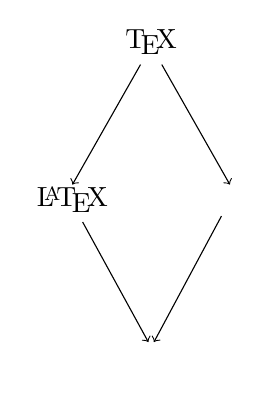
\begin{tikzpicture}
	
	% Les textes
	\node[text height=1ex,anchor=mid] (T) at (0,0) 		 	{\TeX} ;
	\node[text height=1ex,anchor=mid]  (X) at (1, -2)	 	 	{\XeTeX};
	\node[text height=1ex,anchor=mid]  (L) at (-1, -2) 		{\LaTeX};
	\node[text height=1ex,anchor=mid]  (XL) at (0,-4)			{\XeLaTeX};
	
	% Les traits
	\draw[->] (T) -- (X.north);
	\draw[->] (T) -- (L.north);
	\draw[->] (L) -- (XL.100);
	\draw[->] (X) -- (XL.80);
\end{tikzpicture}

\caption{Les relations entre \TeX{}, \LaTeX{}, \XeTeX{} et \XeLaTeX{}}\label{sch:tex}
\end{figure} 

Dans  ce livre nous travaillerons sur \XeLaTeX{}. Toutefois comme la plupart de nos propos peuvent s'appliquer indifféremment  à \LaTeX{} et à \XeLaTeX{}, nous parlerons de \LaTeX{}, sauf lorsque nous signalerons une spécificité de \XeLaTeX{}.

\begin{anedocte}
Bien que le sujet soit controversé, il semblerait qu'il faille prononcer le  \forme{X} de \TeX{} comme un \forme{χ} grec\footnote{\forme{Latek}}, car le nom \TeX{} viendrait du mot grec \forme{\textgreek{τέχνη}} : \forme{art, sciences}.
\end{anedocte}
